\chapter{The South African energy sector}
The Republic of South Africa is one of the most developed country in Africa. SA accounting for about 30~\% of the primary energy consumption and 36.5~\% of the electricity generation of the entire continent Africa in 2013. The primary energy consumption was about 1~425~TWh in total. Therefore the South African society is strongly depend on fossil fuels as primary energy source. As shown in Figure \ref{PEKreis}, coal is with about 72~\% the main primary energy source. Also crude oil (22.2~\%) is a very important energy source for SA. Therefor the primary energy consumption from renewable energies in SA is just about 0.3~\%. Comparing to this, the global share of  renewable primary energy consumption was about 8.9~\% in 2013. The consumption in natural gas is about 2.9~\% which is mainly coming from industrial consumers. 2.6~\% of the primary energy consumption was from nuclear energy in 2013. \cite{BP2014b,Agency2015}
%
\begin{figure}[!h] %Kreisdiagramm Primärenergie
\centering
\def\angle{0}
\def\radius{2.5}
\def\cyclelist{{"brown","orange","yellow","black","green"}}
\newcount\cyclecount \cyclecount=-1
\newcount\ind \ind=-1

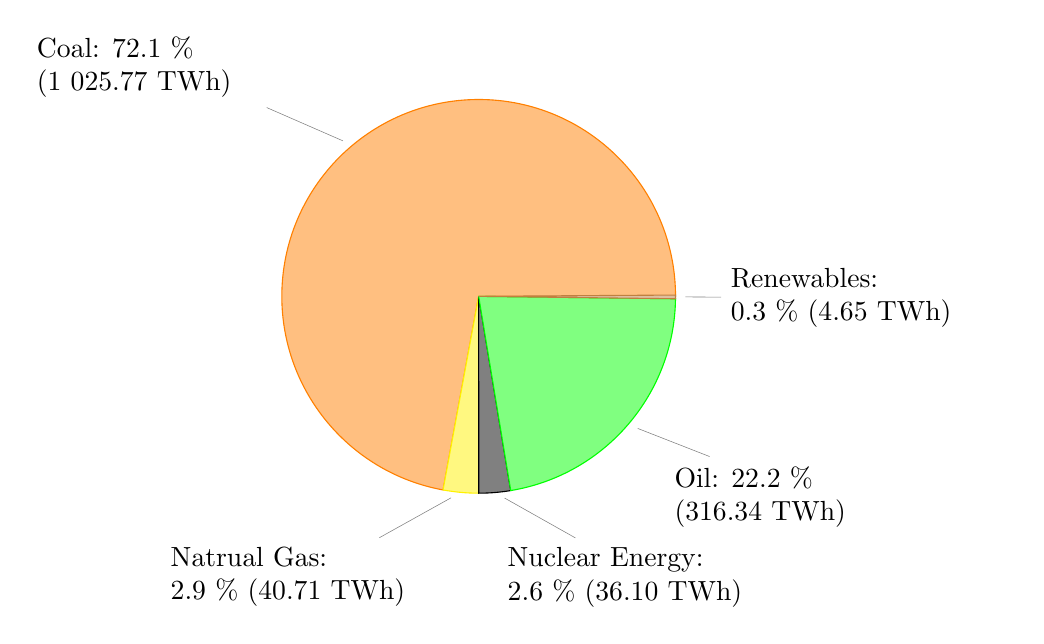
\begin{tikzpicture}
  \foreach \percent/\name in {
      72.1/Coal: 72.1~\% \\(1~025.77~TWh),
  	  2.9/Natrual Gas:\\2.9~\% (40.71~TWh),
      2.6/Nuclear Energy: \\2.6~\% (36.10~TWh),
      22.2/Oil: 22.2~\%\\(316.34~TWh),
      0.3/Renewables:\\0.3~\% (4.65~TWh),
    } {
      \ifx\percent\empty\else                 % If \percent is empty, do nothing
        \global\advance\cyclecount by 1       % Advance cyclecount
        \global\advance\ind by 1              % Advance list index
        \ifnum4<\cyclecount                   % If cyclecount is larger than list
          \global\cyclecount=0                %   reset cyclecount and
          \global\ind=0                       %   reset list index
        \fi
        \pgfmathparse{\cyclelist[\the\ind]}   % Get color from cycle list
        \edef\color{\pgfmathresult}           %   and store as \color
        % Draw angle and set labels
        \draw[fill={\color!50},draw={\color}] (0,0) -- (\angle:\radius) arc (\angle:\angle+\percent*3.6:\radius) -- cycle;
        %\node at (\angle+0.5*\percent*3.6:1.1*\radius) {\percent\%};
        \node[pin=\angle+0.5*\percent*3.6:\parbox{3.5cm}{\raggedright\name}] at (\angle+0.5*\percent*3.6:\radius) {};
        \pgfmathparse{\angle+\percent*3.6}    % Advance angle
        \xdef\angle{\pgfmathresult}           %   and store in \angle
      \fi
    };
\end{tikzpicture}
\caption[Primary energy consumption by fuel excluding solid biomass and waist in South Africa 2013.]{Primary energy consumption by fuel excluding solid biomass and waist in South Africa 2013 \cite{BP2014b}.}\label{PEKreis}
\end{figure}
%


Between 1991 and 2011 the annual primary energy consumption in SA has risen from 996.79~TWh by over 43~\% up to 1~431.01~TWh (excluding solid biomass and waist). Also the annual primary energy consumption per capita rises in the same time period by over 23~\% up to 33.82~MWh per person. Figure \ref{PEV} shows the growing South African primary energy consumption in comparison to primary energy consumption per capita. The Figure shows that not only the population growing but also the rising demand per capita is the reason for the increasing total primary energy consumption in SA.  \cite{BP2014b}
\begin{figure}[htb] % Primary energy consuption 1980-2011
  \centering
  \begin{tikzpicture}
    \pgfplotsset{
        width=\textwidth-45pt,
        height = 0.4\textheight,
        legend style={%
          at={(0.99,0.99)}
        },
        legend pos=north west, 
        legend cell align=left,
        ticklabel shift={0.05cm},
        tick label style={/pgf/number format/1000 sep=},
        xtick={1980,1985,1990,1995,2000,2005,2010},
        x tick label style={rotate=45,anchor=east},
        x tick label style={/pgf/number format/1000 sep=},
        no markers
     }
    \begin{axis}[
        xlabel = {Time [Year]},
        ylabel = {Total primary energy consumption},
        y unit=\si{\tera\watt\hour},
        ymin=600, ymax=1600,
      ]
      \addplot[black] table {Charts/PrimEnergy.csv};
      \label{Primary energy}
    \end{axis}
%
    \begin{axis}[
        yticklabel pos=right,% yticklabel auf der rechten Seite
        ylabel = {Total primary energy consumption per capita},
        y unit=\si{\mega\watt\hour},
        ymin=25, ymax=40,
        xtick=\empty,% xticks nicht noch einmal zeichnen
      ]
      \addplot[red] table {Charts/Total_Primary_Energy_Consumption_per_Capita.csv};
      \addlegendimage{/pgfplots/refstyle=Viskositaet}
      \addlegendentry{Primary energy per capita}
      \addlegendentry{Primary energy}
      \addlegendentry{Primary energy median}
    \end{axis}
  \end{tikzpicture}
  \caption[Total primary energy consumption and total primary energy consumption per capita 1980 to 2011 in South Africa. ]{Total primary energy consumption and total primary energy consumption per capita 1980 to 2011 in South Africa \cite{BP2014b,EIA2015}.}\label{PEV}
\end{figure}

The three major consumption groups are the industry sector with about 34.9~\%, the transport sector which consumes about 28.6~\% and other sectors with about 36.5~\%, which includes agriculture, commerce and public services, residential and non-specified consumers. According to the South African Department of Energy (DoE) was the total final consumption about 738.18~TWh in 2012. \cite{DepartmentofEnergy2012}
\pagebreak
\section{Electricity supply and demand}
Coal-fired power stations restrained the electricity generation in SA. 92.8~\% was generated thought coal (239~344~GWh) in 2012, while 5.1~\% of the annual supply was generated by nuclear power (13~075~GWh) and 1.3~\% was generated from hydropower applications (4~860~GWh). Less significant electricity sources for SA are 0.08~\% Oil (194~GWh), 0.11~\% bio-fuels (293~GWh), 0.02~\% PV (50~GWh) and 0.04~\% wind (103~GWh). \cite{Agency2015}



The final electricity consumption in SA was about 197~092~GWh in 2012. The final consumption consist also three main consumers. The largest consumer group with about 59.5~\% are industrial consumers, followed by residential consumers (19.7~\%) and commercial and public services (14.3~\%). The complete electricity flow is shown in Annexure I, Part A, Table \ref{tab1}, on page \pageref{tab1}. \cite{Agency2015}

\begin{figure}[!h] % Sommer/Winter Verbrauchskurve
\centering
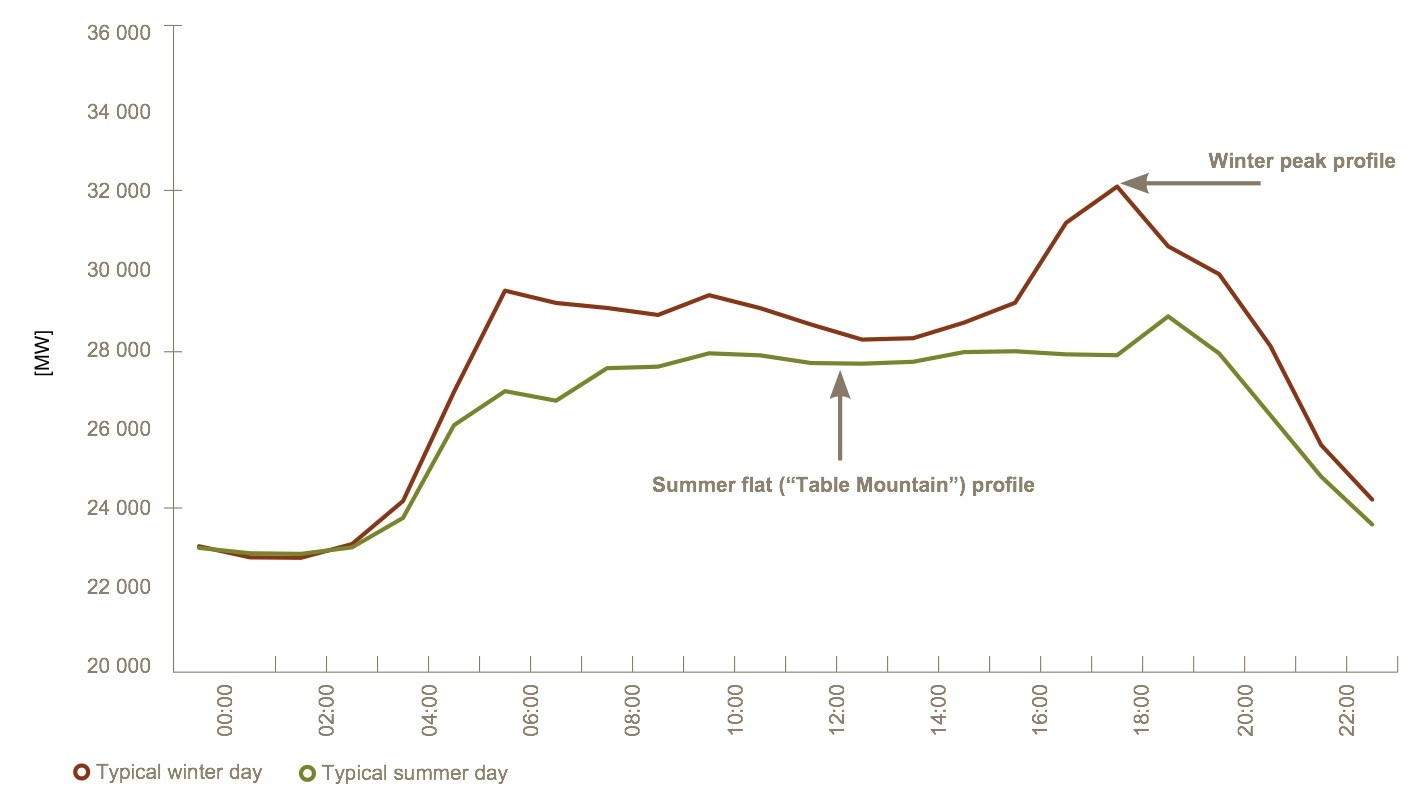
\includegraphics[width=0.9\linewidth]{FIG/SummerWinterDemand}
\caption[Summer and winter load profiles.]{Summer and winter load profiles \cite{Eskom2014}.}\label{DEMAND}
\end{figure}


The demand in South Africa has different load profiles during winter and summer as shown in Figure~\ref{DEMAND}. The peak demand is usually in the evening hours and particularly high during winter time. According to Eskom is the peak demand at about 32~GW, while the usually demand during daytime is between 26~GW and 29~GW. \cite{Eskom2014}

\subsection{Rising energy consumption and security of supply}

\begin{figure}[!h] % Monthly Reserve
\centering
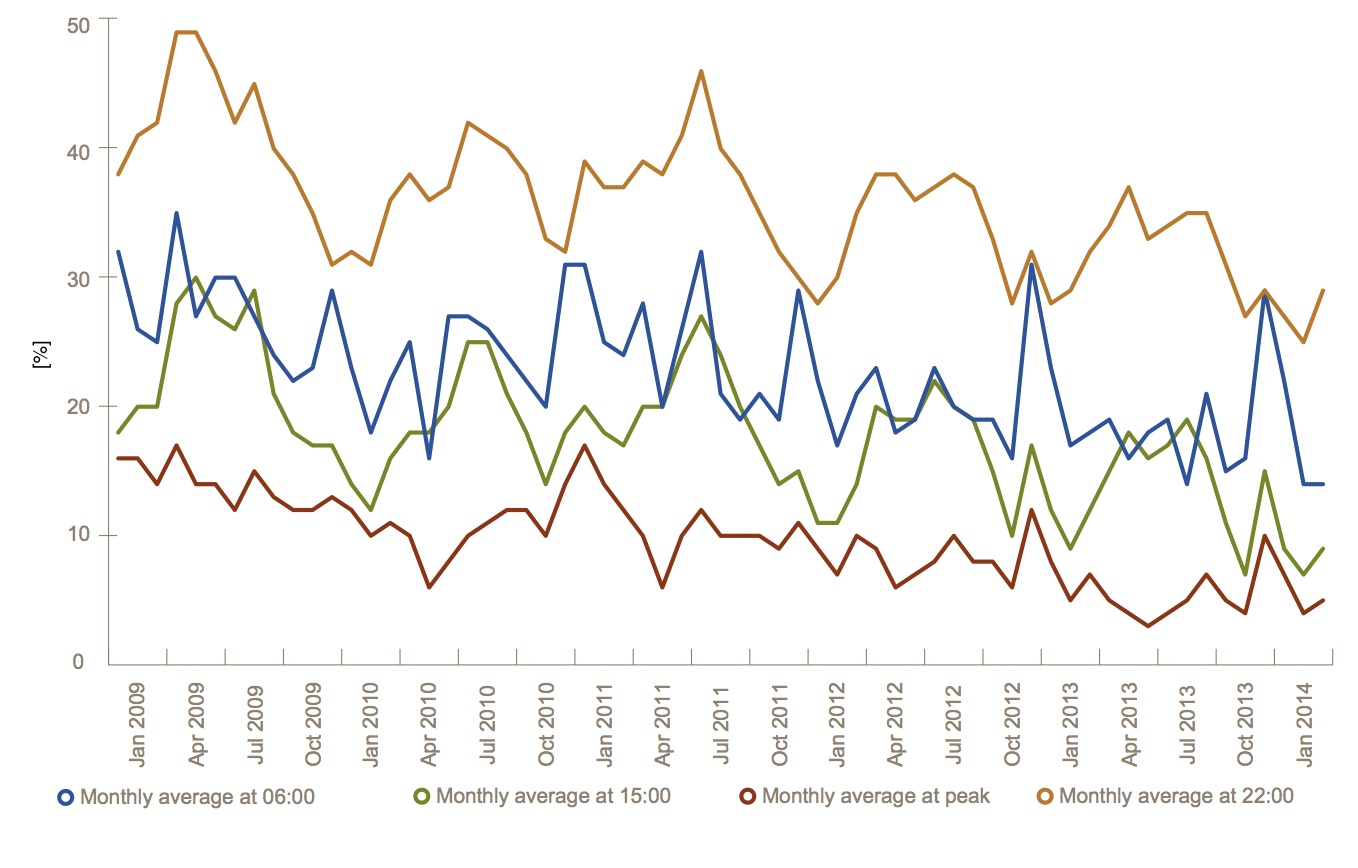
\includegraphics[width=0.9\linewidth]{FIG/AveragemonthlySA}
\caption[Average monthly \% operating reserves.]{Average monthly \% operating reserves\cite{Eskom2014}.}\label{Abb1}
\end{figure}


\begin{figure}[!h] % Demand growth
\centering
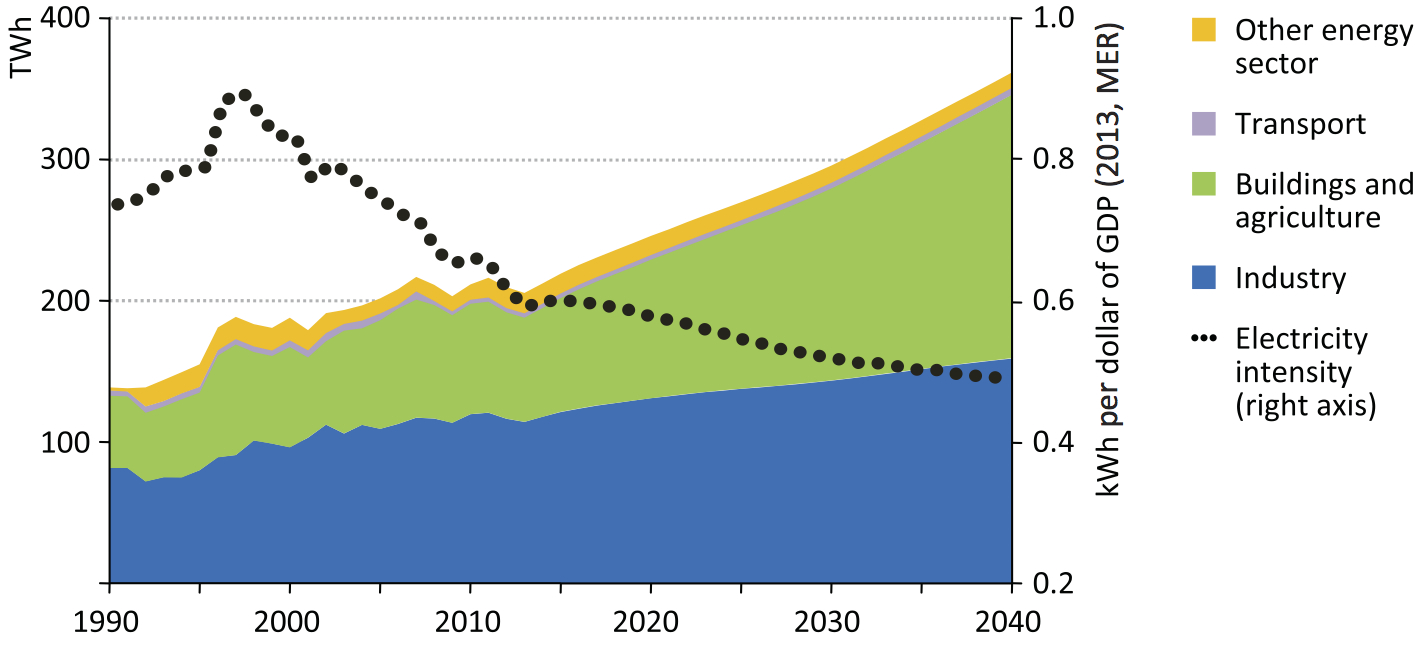
\includegraphics[width=0.9\linewidth]{FIG/SA_Electricity_demand_growth}
\caption[Electricity demand growth by sector in South Africa in the New Policies Scenario.]{Electricity demand growth by sector in South Africa in the New Policies Scenario \cite{IEA2014f}.}\label{Abb1}
\end{figure}

\subsection{Structure of power distribution}
Kilometerlängen, Verluste im Netz \cite{Eskom2014a}

On mainland sub-Saharan Africa, SA has with around 85~\% the highest electrification rate. About 11~\% of households don't have access to electricity and a further 4~\% rely on illegal access (non-paying) or obtain access informally (from one household to another but paying). \cite{IEA2014f}

\begin{figure}[htbp] % Netzstrucktur
\centering
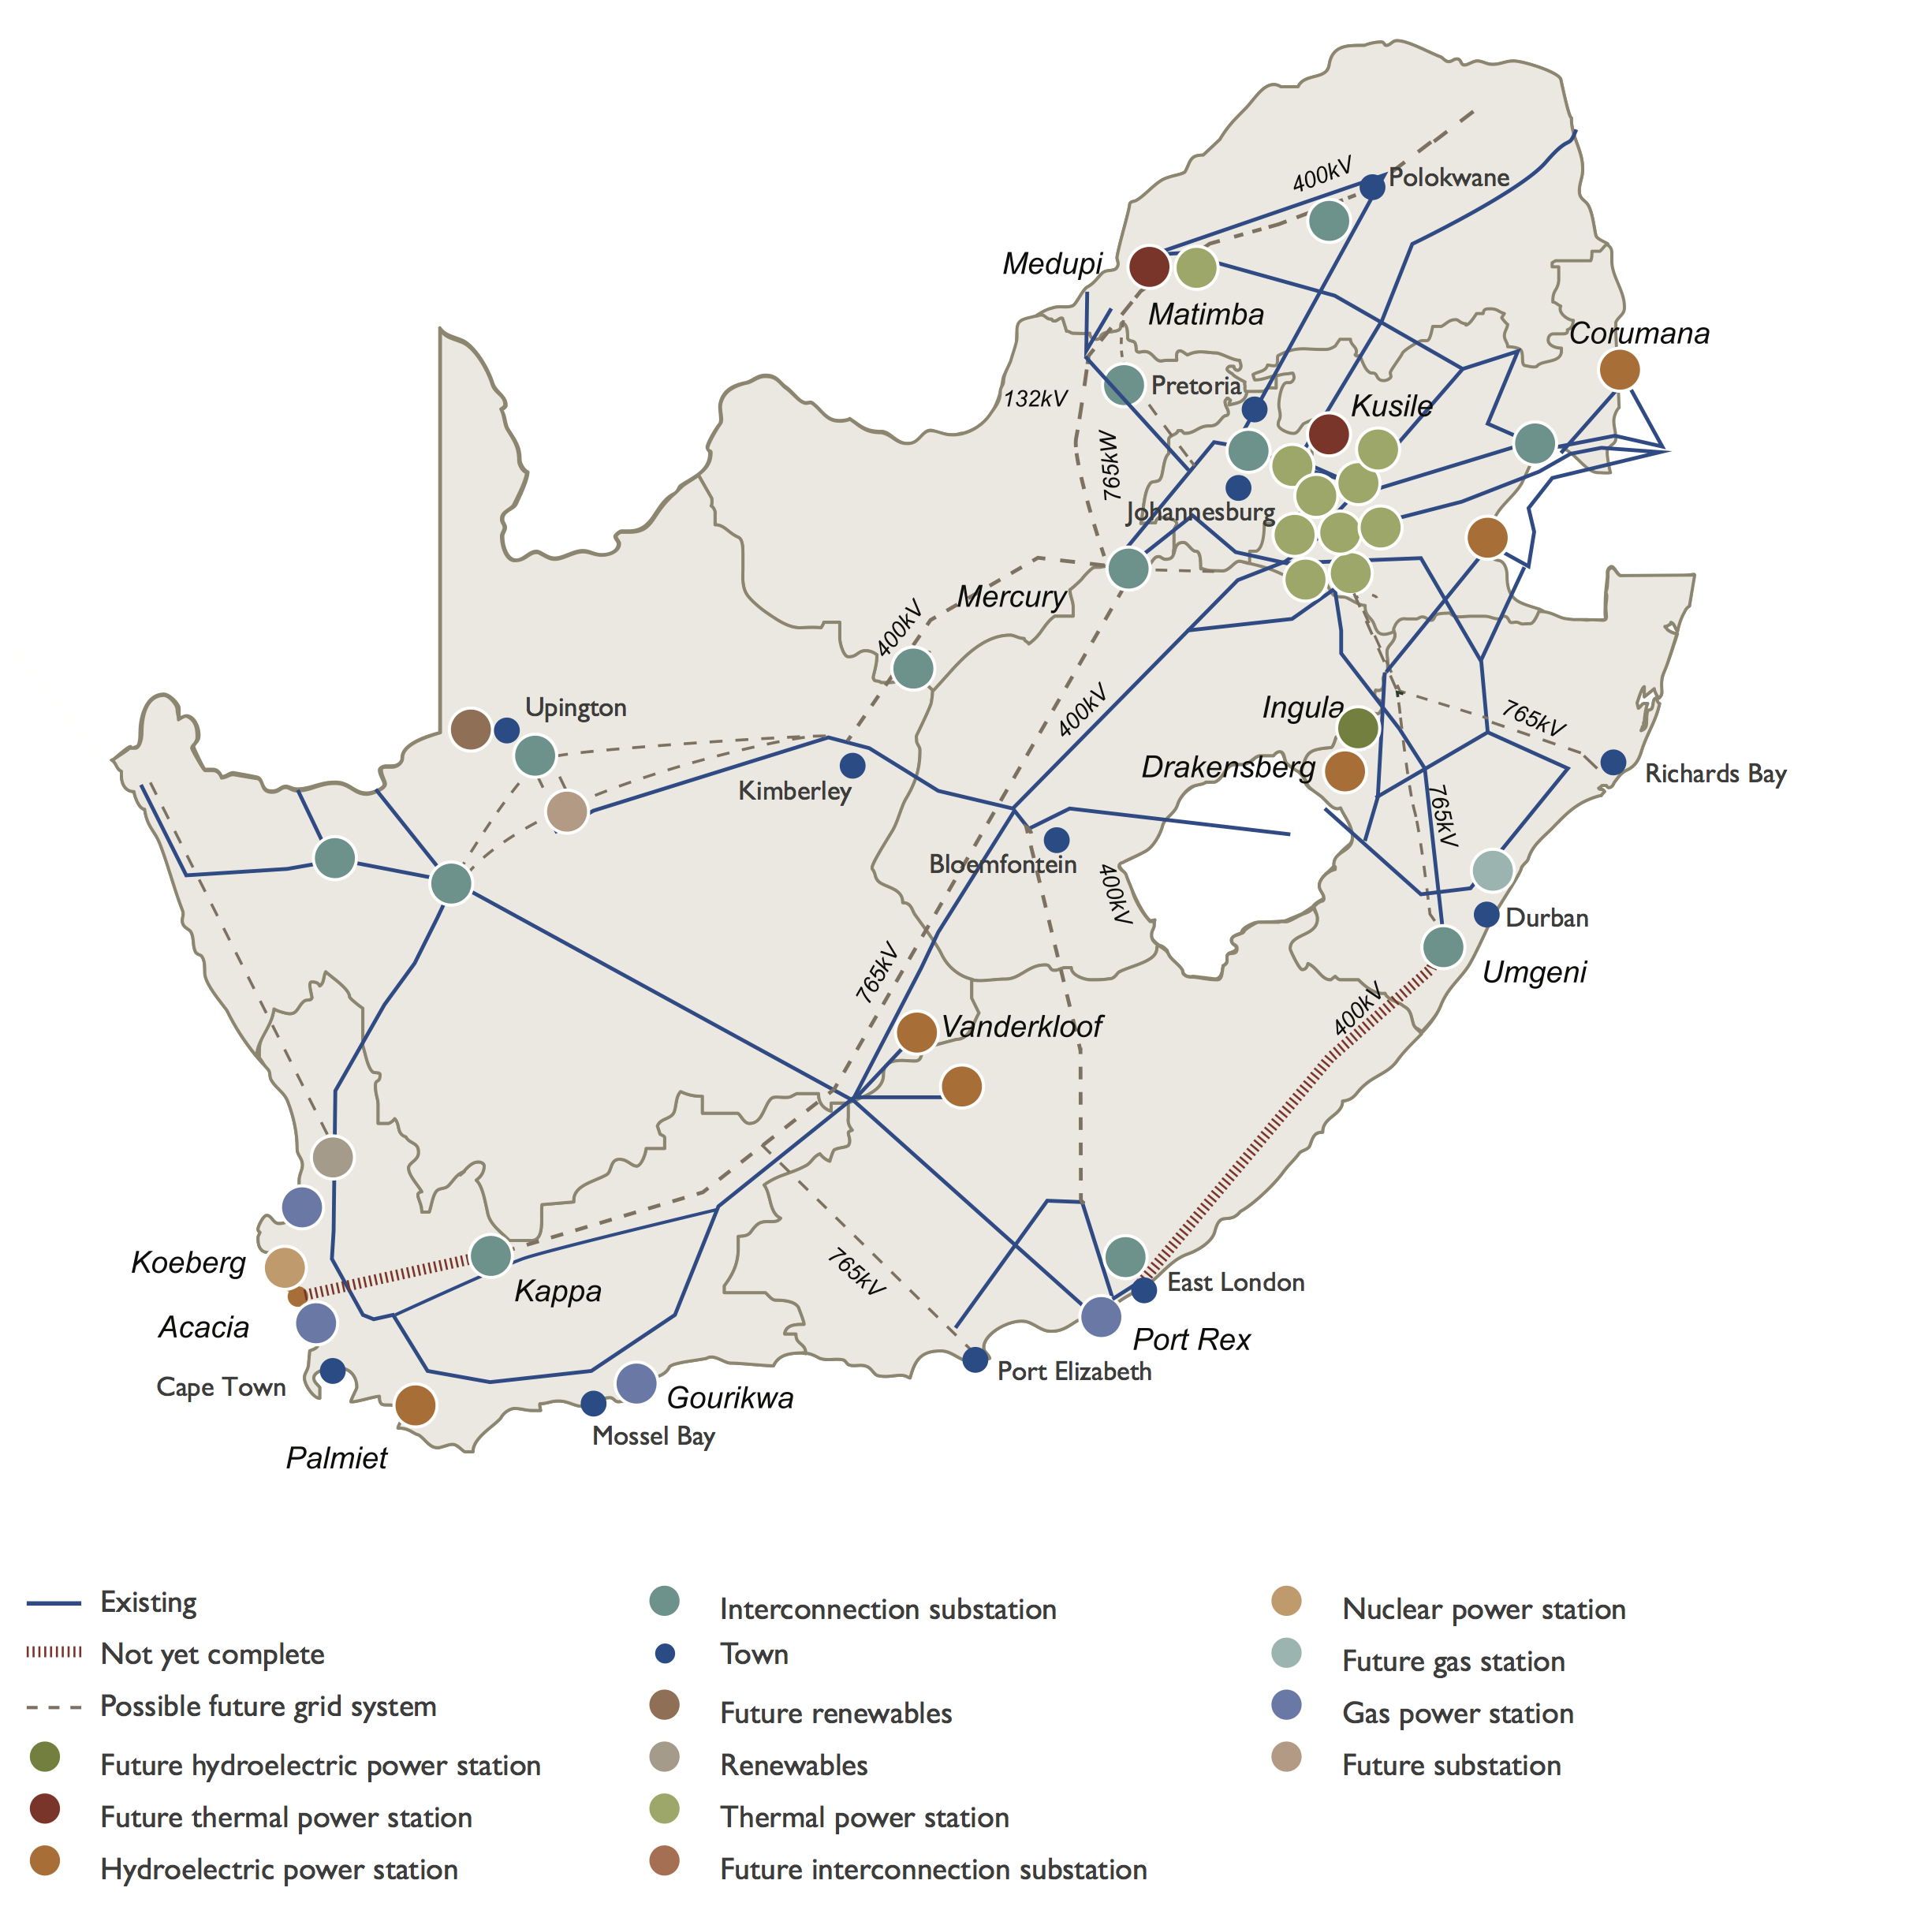
\includegraphics[width=0.9\linewidth]{FIG/transmissionprojekts}
\caption[Eskom’s transmission projects as at 31 March 2014.]{Eskom’s transmission projects as at 31 March 2014 \cite{Eskom2014}.}\label{Abb1}
\end{figure}

http://integratedreport.eskom.co.za/supplementary/app-transmission.php

\section{Renewable energy potential in South Africa}

\subsection{Energy outlook for South Africa}
Development of a Renewable Energy Power Supply Outlook 2015 for the Republic of South Africa
Achieved by Sebastian Giglmayr, BSc
\cite{Giglmayr2013}

\subsection{Government Incentives}

\section{Chapter summary}
\pagebreak
